\chapter{Example Application}

In this chapter I will showcase the development of an example project that aims to demonstrate the capabilities of the selected multicore microcontroller and the Rust programming language. I will highlight features that are plain better from most perspectives, as well as the areas where this approach falls short compared to a traditional C project. The example project will have a definite function but the usage of certain peripherals and language features are more in focus thus the functionality may seem a bit purposeless as a real application.

\section{General Description}

The example application implements a very basic webserver on the M7 core of the microcontroller, and does some light signal processing on the M4 core. The general direction of this project was to design one part of the application to use the ethernet peripheral in some capacity, and the other to be capable of doing a task in real time. Also I had to make sure that safe, two-way communication between the two cores is displayed in the application.

Finally an application draft was drawn up. In it the M7 core handles the ethernet peripheral and takes on the role of a simple webserver. It hosts a simple website on a fixed IP address where coefficients of a low pass filter can be supplied. The site also displays the average value of an ADC peripheral. The other core handles the previous ADC peripheral by performs filtering with the coefficients supplied on the website and a fix formula. The filtered signal is emitted on a DAC peripheral with minimal latency latency. An average value is also calculated by the M4 core periodically from a configurable number of samples, this value will be displayed on the website.

\begin{figure}[!ht]
    \centering
    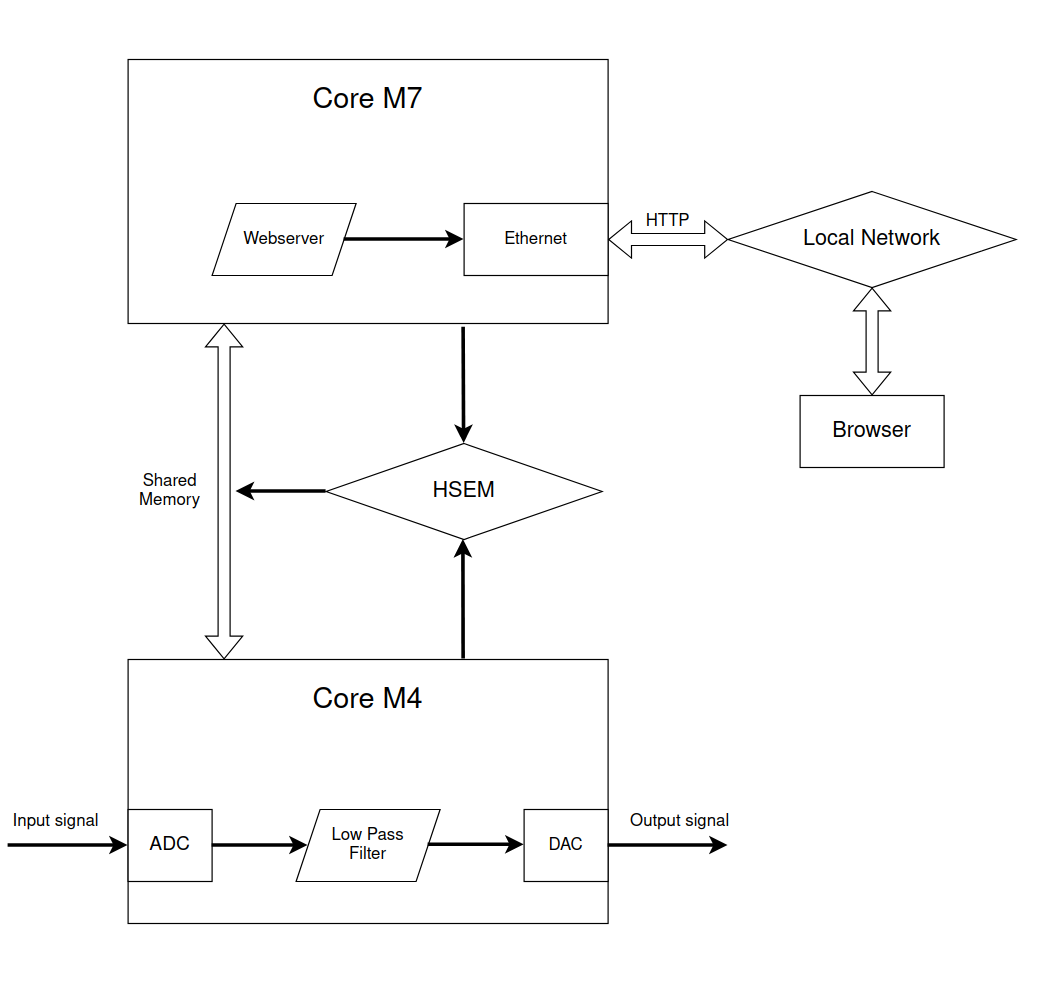
\includegraphics[width=150mm, keepaspectratio]{figures/example-app-flowchart.png}
    \caption{Block Diagram of the Example Application}
    \label{fig:hsem-interrupt-sd}
\end{figure}

With this flow, the application demonstrates the usage of  a decent number of peripherals, namely an ADC, a DAC, ethernet, UART and LEDs for debugging, and of course the hardware semaphores for preventing concurrent shared memory access.

\section{Peripherals}

This section demonstrates the initialization and usage of the peripherals mentioned above. Although most of these were already introduced in the previous chapter this section will focus on specific settings that facilitate this example application.

\subsection{Basic peripherals}

The basic peripherals and their usage, namely UART, LEDs, and shared memory, are already well documented in previous chapters. However some significant changes were done to the very beginning of the program where clocks, resets, and power sources are initialized. This was necessary for two reasons. For once, different clock and reset configuration was needed if we were to use the ethernet peripheral, it needed multiple types of clock signals which are supposed to be related to each other in value. The second reason was an issue where resetting the system caused it to go into an unsteady state and behave unexpectedly, eg. only one core would work. This state could only be fixed by loading a new image onto the microcontroller.

\begin{lstlisting}[language=Rust,frame=single,float=!ht,style=customrust,label={lst:clock-config},caption={Initialization of Clocks, Resets, and Power Sources}]
    let pwr = dp.PWR.constrain();
    let pwrcfg = pwr.smps().vos0(&dp.SYSCFG).freeze();

    // link SRAM3 power state to CPU1
    dp.RCC.ahb2enr.modify(|_, w| w.sram3en().set_bit());

    // Enable HSEM clk
    dp.RCC.ahb4enr.modify(|_, w| w.hsemen().set_bit());

    let rcc = dp.RCC.constrain();
    let mut ccdr = rcc
        .sys_ck(200.MHz())
        .pll1_strategy(rcc::PllConfigStrategy::Iterative)
        .pll3_p_ck(PLL3_P)
        .hclk(200.MHz())
        .pll1_r_ck(100.MHz())
        .freeze(pwrcfg, &dp.SYSCFG);

    _cp.SCB.invalidate_icache();
    _cp.SCB.enable_icache();
    _cp.DWT.enable_cycle_counter();

    assert_eq!(ccdr.clocks.hclk().raw(), 200_000_000); // HCLK 200MHz
    assert_eq!(ccdr.clocks.pclk1().raw(), 100_000_000); // PCLK 100MHz
    assert_eq!(ccdr.clocks.pclk2().raw(), 100_000_000); // PCLK 100MHz
    assert_eq!(ccdr.clocks.pclk4().raw(), 100_000_000); // PCLK 100MHz
\end{lstlisting}

In Listing~\ref{lst:clock-config} power is enabled in the usual way, then clock and power is enabled for the SRAM3 memory, which will be used by the ethernet driver, and the hardware semaphores. Then the clocks are configured according to ethernet examples from the \mycode{stm32h7xx-hal} crate. \cite{HalExamples} After that the instruction cache is flushed and enabled so every restart starts the MCU with a clean state in this regard. The last section asserts that all the clock signals are correctly configured for ethernet usage. Debugging issues around clocks would be a frustrating task when the code is already developed, so it is imperative that these asserts stop the execution if the clocks are incorrectly configured.

Some of the variable names are prepended with an underscore which signals to the Rust compiler that the variable is intentionally left unused. This may seem strange especially when a variable like this is used, but we have to remember that the code for the two diverge at some point and become separated at compile time. So if a variable is not used on one core, it will generate a warning even if the other core uses it. This solution is more acceptable then turning off unused variable warnings altogether.

\subsection{Ethernet}

In this section I will demonstrate the usage of the ethernet peripheral and its driver coupled with a TCP stack.

\subsubsection{Driver}

The ethernet driver is part of the \mycode{stm32h7xx-hal} crate. this driver provides an interface for the STM32H7 microcontroller to communicate over Ethernet using the MAC and PHY components. It leverages DMA for efficient data transfer and integrates with the \mycode{smoltcp} crate, which will serve as the TCP stack, to enable networking capabilities. The driver can be used for tasks such as sending and receiving Ethernet frames, configuring MAC and PHY parameters, and interfacing with higher-level networking protocols.

The driver provides an \mycode{EthernetMAC} struct which represents the MAC (Media Access Control) layer. It initializes and configures the MAC for communication by setting up its registers. These hold various information handled by this layer such as MAC address and flow control settings. It also provides methods \mycode{smi_read()} and \mycode{smi_write()} for the SMI (Serial Management Interface) which facilitates the communication between the MAC and the external PHY registers. these methods are provided by implementing the \mycode{StationManagement} trait for the \mycode{EthernetMAC} struct.

DMA is extensively used by the ethernet driver so the CPU is not throttled by the constant flow of information that is typical to this interface. The \mycode{EthernetDMA} struct represents the Ethernet DMA engine which is responsible for managing the flow of data between memory and the MAC.
DMA descriptors, \mycode{TDes} and \mycode{RDes}, are used to control the transfer of data between the MAC and memory. The descriptors are organized in rings for efficient handling of multiple data frames. The \mycode{TDesRing} and \mycode{RDesRing} structs manage the transmit and receive descriptor rings, respectively. The \mycode{init()}, \mycode{available()}, \mycode{release()}, and \mycode{buf_as_slice_mut()} methods provide functionality for initializing, checking availability, releasing, and accessing DMA descriptors and associated buffers.

\subsubsection{Smoltcp}

The smoltcp crate stands as a versatile networking stack in the Rust programming language, designed to offer modularity and composability for the development of networking applications. At its core, smoltcp supports a range of essential networking protocols such as IPv4, IPv6, TCP, UDP, ICMP, and more. In this project, smoltcp is primarily used as a TCP stack in the networking schema. \cite{Smoltcp}

One of the key architectural principles of smoltcp lies in its abstraction of networking devices through the \mycode{phy::Device} trait. This trait serves as the interface for network devices, allowing seamless integration with different hardware or software networking implementations. This level of abstraction enhances the adaptability of smoltcp to various platforms and facilitates ease of use.

A notable aspect of the crate is its adherence to the Berkeley Sockets API, providing a familiar programming interface for developers well-versed in network programming. This socket API simplifies the process of building networking applications, contributing to a smoother development experience.

Still, one of the main reasons smoltcp is used in embedded projects like this is that is can operate using a \mycode{no_std} environment, and still being able to provide fairly high level API-s.

\subsubsection{Connection to TCP stack}



\subsection{ADC}

\subsection{DAC}


\section{Setup Phase}


\section{Main Loop}

\subsection{Webserver}

\subsection{Signal Filtering}
